\documentclass[
    bindingoffset=5mm,  % Binding offset
    footnoteindent=3mm, % Footnote indent
    hyphenation=true    % Hyphenation turn on/off
]{tpl/wut-thesis}

\graphicspath{{src/img/}} % Images directory
\addbibresource{bibliography.bib}

\facultyeiti
\EngineerThesis
\langeng

\begin{document}

%------------------
% Title page
%------------------
\institute{TODO: Institute}
\fieldofstudy{TODO: Telecommunications?}
\specialization{TODO: Specialization}
\title{
  TODO: Thesis title
}
% Polish title
\poltitle{
  TODO: Tytuł pracy po polsku
}
\author{Błażej Sewera}
\studentnumber{300499}
\supervisor{mgr inż. Maciej Sosnowski}
\date{2022}
\maketitle

%-------------------------------------
% English abstract
%-------------------------------------
\cleardoublepage % Starting from an odd page
\abstract TODO: Abstract
\keywords XXX, XXX, XXX

%----------------------------------------
% Polish abstract
%----------------------------------------
\clearpage
\secondabstract TODO: Streszczenie po polsku
\secondkeywords XXX, XXX, XXX

\pagestyle{plain}

%--------------
% Table of Contents
%--------------
\cleardoublepage
\tableofcontents

%------------
% Sections
%------------
\cleardoublepage
\pagestyle{headings}

\clearpage
\section{Project management}\label{sec:project-management}

One of the biggest challenges turned out to be non-technical.
Project management,
even with only one person can be difficult,
as it requires a lot of self-discipline.
Luckily, there were some tools and processes that helped with this task.

\subsection{Project setup}\label{sec:project-setup}

Before starting a project,
we know the least about it.
We want to make the least decisions
at this point~\cite{beck_extreme_2004,erder_principle_2016}.
The things most susceptible to change
should be~considered to be changed in the future.
It is of utmost importance to capture
the essence of the problem.
\Ac{DDD} helps with
gathering this essence,
which is called
the core domain~\cite{millett_patterns_2015}.
The domain of Notipie is described in detail
in section~\ref{sec:domain}.

On the other hand,
we have to be aware that our application
may not necessarily be suitable for \ac{DDD} patterns.
I also took care for the simplicity
of every aspect of~my application,
so that when I sat to read the code
I wrote six months before,
I~was able to understand it
within a reasonable time.

\subsection{Product development}\label{sec:product-development}

The most important thing
I learned in the field of project management
was undoubtedly how to reliably conduct product development.
When I started developing Notipie,
I had a very vague vision
of what the finished product will provide.
The essential functionality was interleaved with features
that could not be implemented without the essentials.

That is when I decided to streamline the development
and set a constraint of what needs to be done
in order to consider the product usable.
I defined the \textbf{Minimum Viable Product}.
I also prioritized the issues
based on the MVP~\cite{sewera_issues_2022}.
More on this topic in section~\ref{sec:minimum-viable-product}.

\subsection{Project board}\label{sec:project-board}

One of the great tools that helped with the project management
was the new Github Projects app,
depicted in figure~\ref{fig:github-projects-kanban},
which was in beta stage
when I started to use it~\cite{github_inc_github_2022}.
The Kanban board~\cite{goddard_kanban_2022} consists of four sections (columns):

\begin{itemize}
      \item
            \textit{Todo} -- which consists of all the issues
            connected to this project
            that are planned to be worked on in the future,
      \item
            \textit{Open} -- which consists of issues
            that need to be worked on next.
            Those are usually one to three issues
            that need to be done in a certain order,
      \item
            \textit{In Progress} -- which contains issues
            that are currently being worked on.
            There is usually only one issue in this column,
      \item
            \textit{Done} -- which consists of all the finished issues,
            as well as the issues that were deemed unnecessary,
            in which case, they are labeled ``won't fix''.
\end{itemize}

Another convenient tool in the same Github Projects app
was the table view.
I~configured one of the table views to present a Backlog,
a list of issues in the whole project,
which I could manually sort by
issue priority and urgency
so as to enable quick progress overview.
The Backlog view is presented in figure~\ref{fig:github-projects-backlog}.

\begin{figure}[!h]
      \centering
      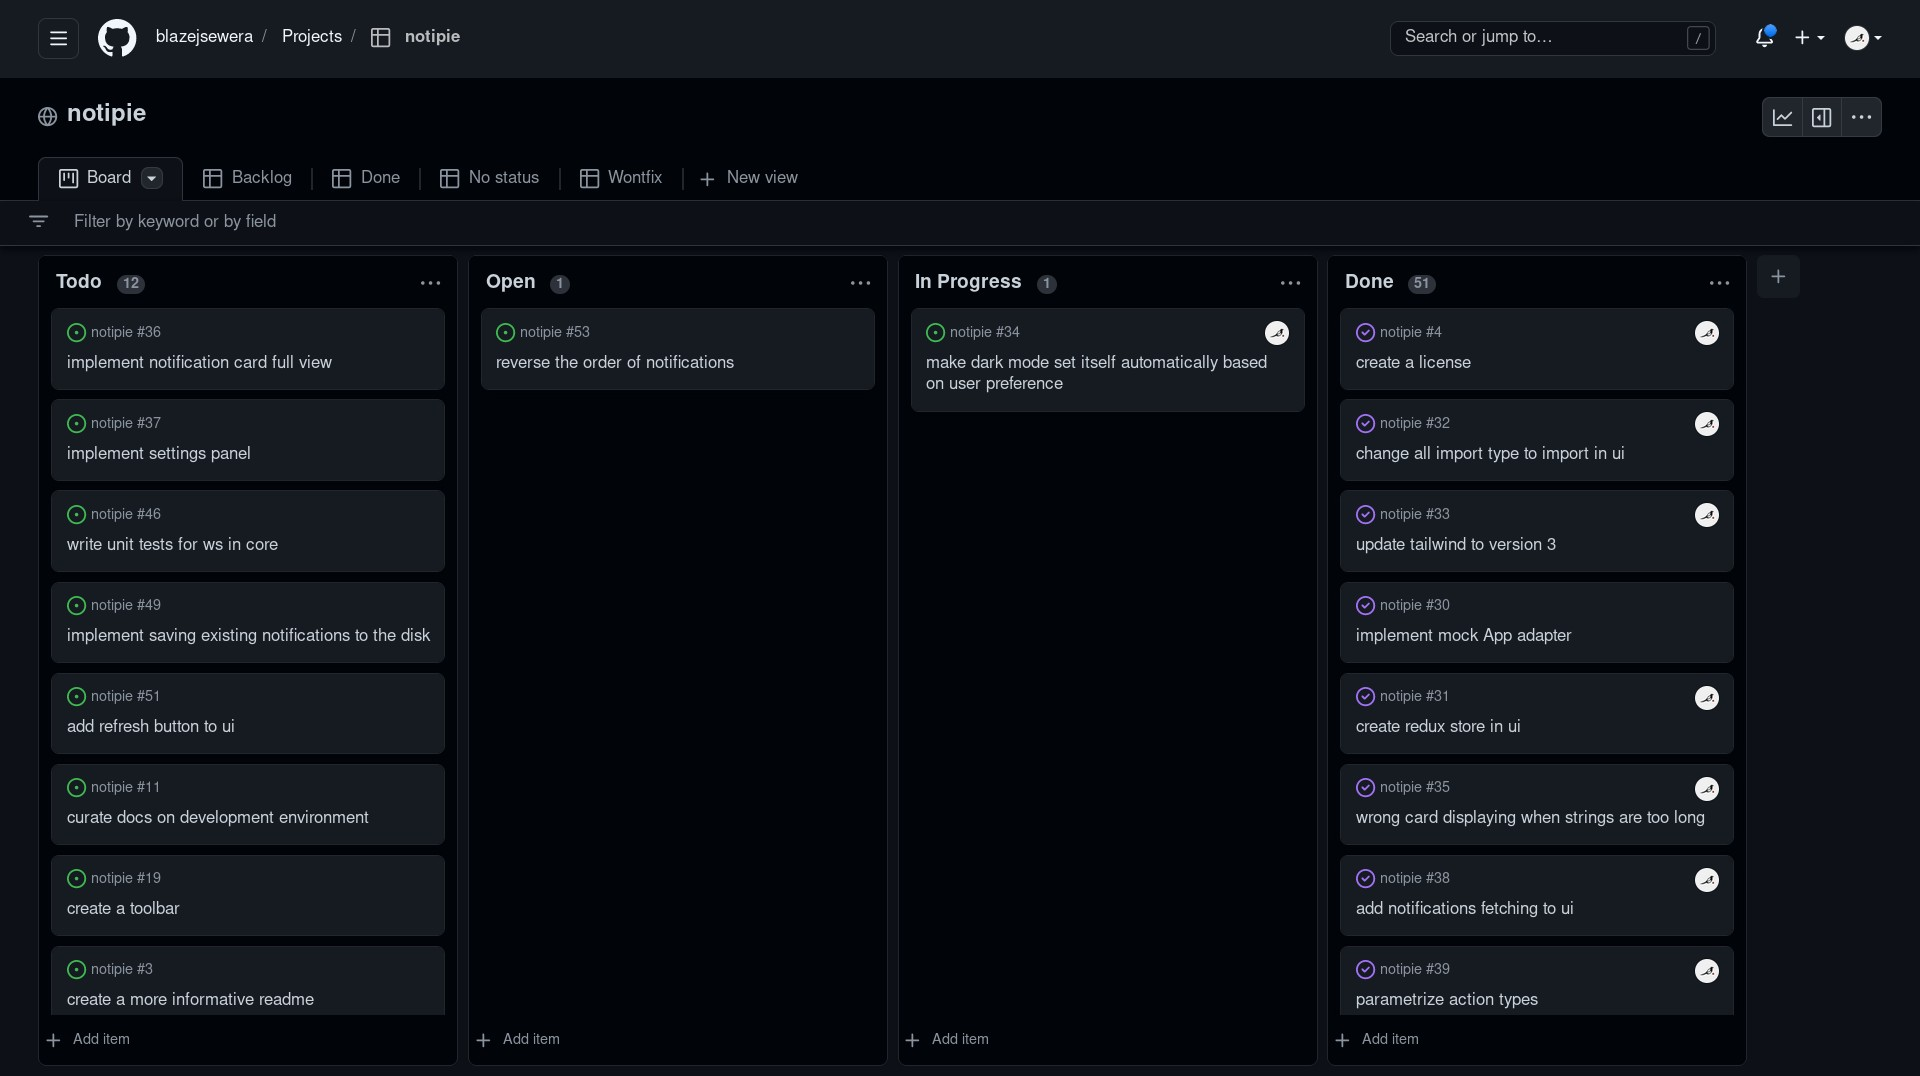
\includegraphics[width=0.99\linewidth,keepaspectratio]{img/kanban_board.jpg}
      \caption{Github Projects: Kanban board view}
      \label{fig:github-projects-kanban}
\end{figure}

\begin{figure}[!h]
      \centering
      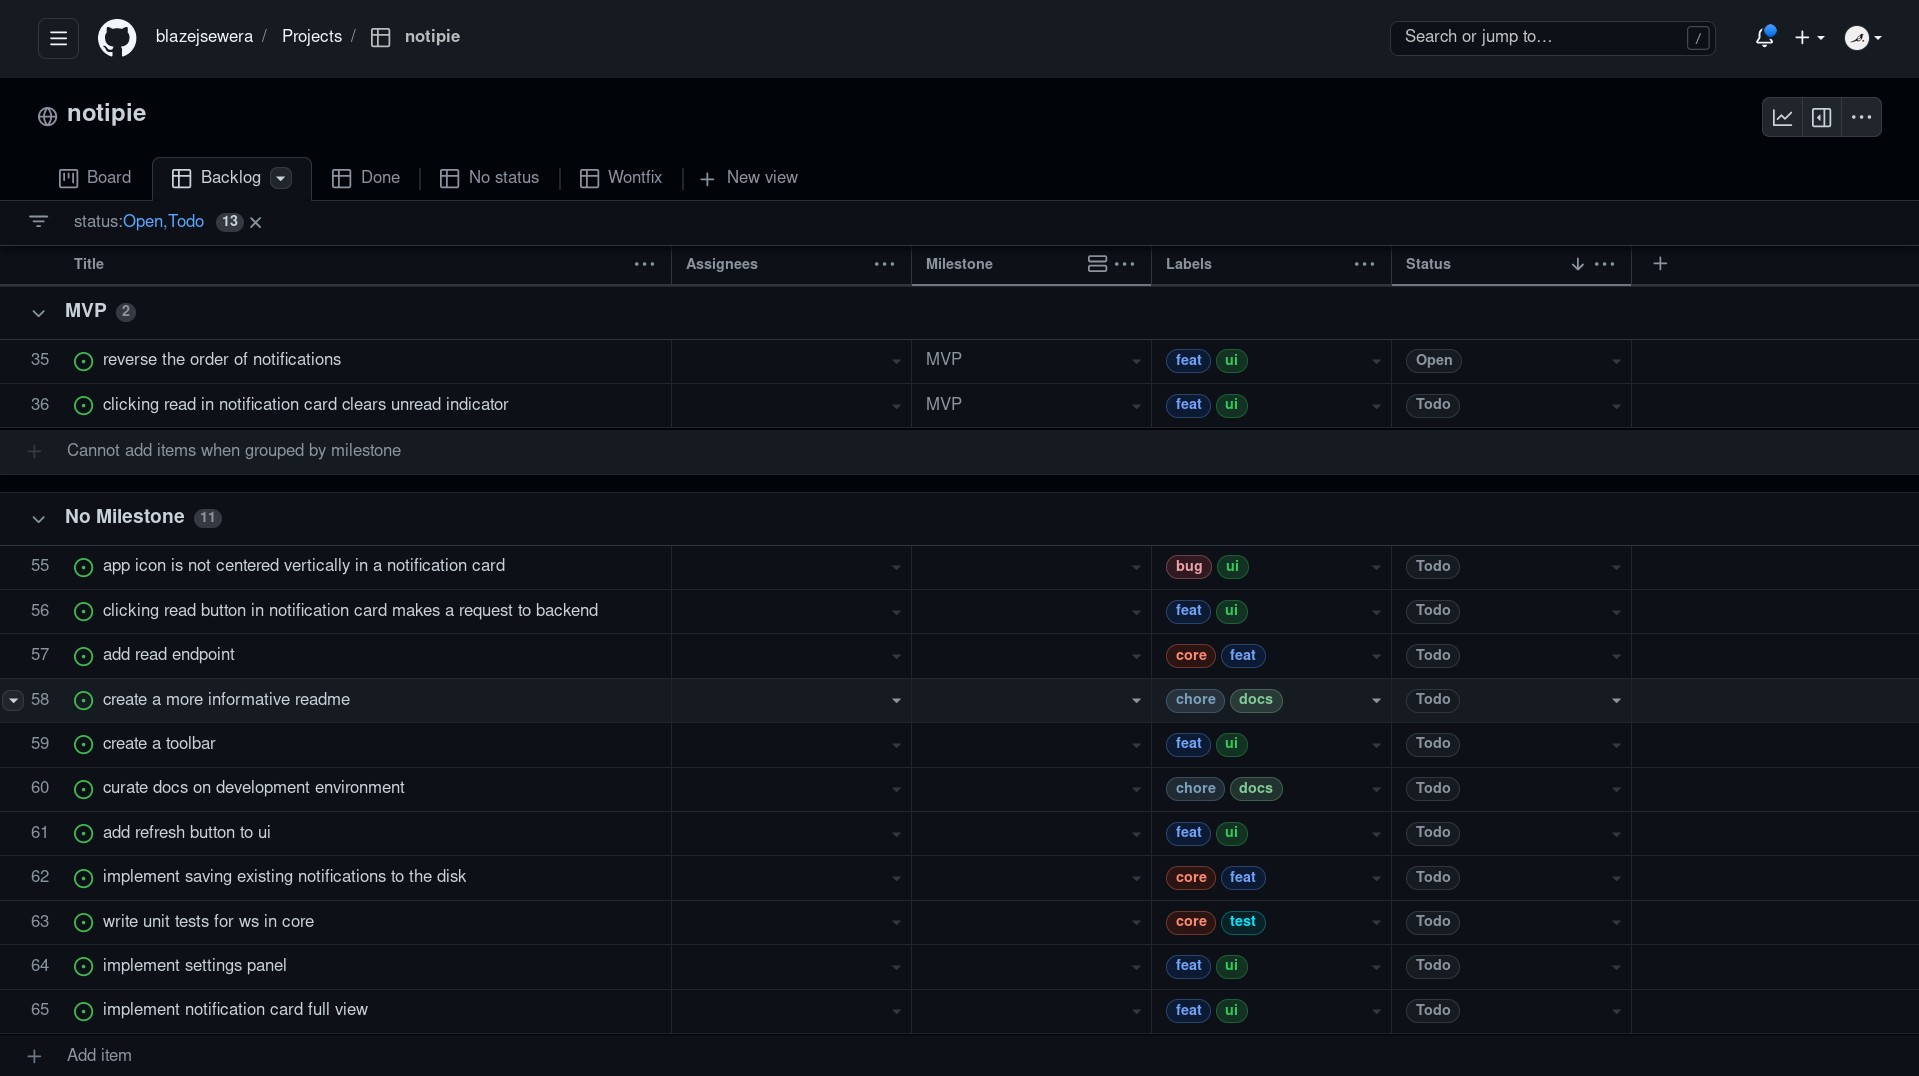
\includegraphics[width=0.99\linewidth,keepaspectratio]{img/backlog.jpg}
      \caption{Github Projects: Backlog view}
      \label{fig:github-projects-backlog}
\end{figure}



\clearpage
\section{Backend}\label{sec:backend}

The backend is a component in a system
that is responsible for the data processing.
It interacts with the frontend applications
with a well-known protocol,
usually one understood by a browser.
Splitting the system into frontend and backend
enables easier reuse of the business logic,
and writing different frontend applications
that use the same backend.
Many huge organizations practice splitting
their systems into frontend and backend.
An example of this is Facebook,
which benefits from the ability to use
many different languages and libraries
that can interact between one another~\cite{abdullah_frontend_2014}.

The backend of Notipie
needed to be both performant,
easy to deploy,
and well-tested.
I strived to make use of the best practices
in the field of microservices,
maintain great quality,
and ensure sufficient performance.
I named it \textit{core},
because there can be different UIs,
or notification producers,
but the entire application's core
is specifically the backend implementation.
The backend code
is in the
\texttt{core} directory~\cite{sewera_notipie_2022}.

\subsection{Core project architecture}\label{sec:core-project-architecture}

An overview of the backend architecture
from the asynchronous notification flow perspective
is presented in figure~\ref{fig:high-level-backend-flow}.
The project on the top-level is structured over 4 directories,
named according to
the \citetitle{quest_standard_2022}~\cite{quest_standard_2022}:

\begin{figure}[h]
      \centering
      \includegraphics[width=6.5cm,keepaspectratio]{chart/out/backend-flow.pdf}
      \caption{Backend architecture for asynchronous notification flow}
      \label{fig:high-level-backend-flow}
\end{figure}

\begin{itemize}
      \item
            \texttt{cmd} -- entry point to the application (\texttt{main})
      \item
            \texttt{internal} -- application-specific code
      \item
            \texttt{pkg} -- reusable utils, not specific to the application
      \item
            \texttt{test} -- black box integration test code
\end{itemize}

\subsubsection{The internal directory}\label{sec:the-internal-directory}

Application-specific code is split into 5 directories
representing the levels of abstraction:

\begin{itemize}
      \item
            \texttt{domain} -- business logic,
            defines data structures and communication of domain objects
            on the highest level of abstraction,
      \item
            \texttt{grid} -- lower level of abstraction than domain,
            defines proxies that convert network models into domain models,
            and connects those proxies with the domain components,
      \item
            \texttt{impl} -- implements network endpoints,
            WebSockets, and persistence,
      \item
            \texttt{infra} -- configures the application
            and sets up the context for DI.
\end{itemize}

There also was a \texttt{model} package
in the \texttt{internal} directory,
but I moved it to an exportable \texttt{pkg} directory,
to reuse it in the notification producer.

\subsubsection{Grid}\label{sec:grid}

The grid is an application layer
that connects implementations of
the endpoints, WebSockets, and persistence
with the domain objects.
I decided to define that name in the UL
to mean this exact intermediate layer.
The name itself was inspired by a power grid
which connects components
from power generation
to appliances.

The implementation is based on the proxies
for domain Apps and Users\footnote{
      The App and the User are defined in
      sections~\ref{sec:app}~and~\ref{sec:user}
      respectively.
}.
Those proxies convert the applicable network models
and perform intermediate procedures
that do not concern the domain,
like Notification ID generation.

This layer is especially important
to keep the domain clean and concise
and to enable easy replacing\footnote{
      The differences between writing code
      for reuse and replacement are described in detail
      in section~\ref{sec:code-quality}.
}
of concrete implementations.

\subsection{Go in core}\label{sec:go-in-core}

Go is quickly gaining popularity among developers,
with its great tooling
and a state-of-the-art standard library.
It is an excellent language for writing microservices.
Its focus on this one task
and pragmatism in adding features to the language by its authors,
resulted in an easy to understand and use,
yet very powerful set of tools.

\subsubsection{Motivation}\label{sec:motivation}

When choosing the right language for the project,
I focused on finding the right tool
for the application and developer experience.

I wanted \texttt{notipie} to be a high-performance microservice,
so I did not take interpreted languages
like Python or JavaScript into consideration.
I mostly considered Java, Kotlin, Rust, and Go.

Java, although popular, does not have the greatest developer experience.
Things like \texttt{equals} and \texttt{hashCode}
are unnecessary bloat in the code.
Project Lombok~\cite{zwitserloot_project_2022} fixes some of them,
but the tooling is limited to IntelliJ,
you have to download a lot of libraries for dealing with JSON,
create your own code style guide,
and perform a fair bit of setup.

Kotlin, far better than Java,
but also locked-in to IntelliJ with tooling,
was an interesting option for me, but not ideal.

Rust was too low-level for my application.
Explicit memory management, although performant,
was simply too verbose and work-intensive for my use case.

Go was a perfect option.
A plethora of great tooling,
like first-party Go plugin for VSCode, GoLand from JetBrains,
community plugins for Neovim,
all working great and providing a good developer experience.
Furthermore, extraordinary performance of the tooling itself,
with tests running in under a second, super-fast compiler,
one of the best standard libraries I have seen,
and overall simplicity of the language, made the choice obvious.

\subsubsection{How did Go make the development easier}\label{sec:how-did-go-make-the-development-easier}

\paragraph*{Built-in language features}\label{par:built-in-language-features}

The features that helped the most during development
were channels and \emph{goroutines},
coroutines automatically managed by the Go runtime.
The idea behind those was very simple to understand,
and working with concurrent programming was a lot easier.

\paragraph*{Goroutines and channels}\label{par:goroutines-and-channels}

Among of the best features of the Go language lay goroutines and channels.
They make concurrent programming a lot easier, compared to other languages.
I used both goroutines and channels
for inter-object communication in \texttt{domain} package.

For example, in {tag.go}~(appendix~\ref{apx:concurrency-in-go}),
after the Tag object is created,
the constructor calls
the \texttt{start} method~(listing~\ref{lst:start-method-in-tag}).
It is running a new goroutine for every Tag instance,
enabling them to asynchronously communicate with other objects.

The Tag was a particularly special case,
in which I had to solve
the Notification duplication problem,
described in detail in section~\ref{sec:tag-technicalities}

\paragraph*{Standard library}\label{par:standard-library}

Standard \texttt{testing} package~\cite{cox_testing_2022} provided
a unified, and simple tooling for testing.
I did not have to think anything about test setup.
No custom scripts, third-party libraries, or IDE setup.
All I needed to do was to name a file with a \texttt{\_test.go} suffix,
write a function starting with \texttt{Test},
and run \texttt{go\ test\ ./...}.
Both VSCode with Go plugin and GoLand
automatically picked up the test setup,
and I was ready to develop with TDD.

Standard \texttt{net/http} package~\cite{cox_http_2022} provides everything
needed for setting up REST endpoints.
Although I used Gin~\cite{martinez-almeida_gin_2022} for this,
due to a simpler interface,
I used status codes and HTTP client implementation from \texttt{net/http}.

\paragraph*{Refactoring to the standards}\label{par:refactoring-to-the-standards}

During this project,
I refactored my functions to better suit
the Go standard library.

For instance,
in commit \texttt{00547cd}\footfullcite{sewera_chorecoreproducer_2022},
I refactored the \texttt{ToJSON} method
to better suit the standard signatures
(appendix~\ref{apx:method-signature-refactoring-in-go}),
i.e. to return the byte array and error,
just like the \texttt{Marshal} method
from the \texttt{json} package~\cite{cox_json_2022}
in the standard library.

\paragraph*{Third-party libraries}\label{par:third-party-libraries}

Gin was great for writing REST endpoints,
with \texttt{gin.Context} having easy access to
standard-library-compatible fields,
making it easily pluggable to other third-party libraries,
like Gorilla WebSocket~\cite{burd_gorilla_2022}.

Zap~\cite{shah_zap_2022} provided a reliable
and performant way to log things in the backend.
Structured logging,
straightforward syntax,
automatic serialization to JSON in production mode,
and human-readable format in debug mode,
paired with low or zero-allocation overhead,
made it a perfect choice for logging in a microservice.

\addtocategory{commit}{sewera_chorecoreproducer_2022}

\subsection{The benefits of using Go}\label{sec:the-benefits-of-using-go}

\subsubsection{Built-in language features}\label{sec:built-in-language-features}

There were numerous features
that helped during backend development.
Implicit encapsulation of functions and variables
starting with a lowercase letter,
structure field annotations
enabling easy serialization
to JSON and YAML,
coroutines automatically managed by the Go runtime,
or channels,
just to name a few.
The idea behind most of them
was very simple to understand,
the usage was intuitive,
and I did not have to resort to the documentation that often.

\subsubsection{Goroutines and channels}\label{sec:goroutines-and-channels}

Among of the best features of the Go language lay goroutines and channels.
They make concurrent programming a lot easier, compared to other languages.
I used both goroutines and channels
for inter-object communication in \texttt{domain} package.

For example, in {tag.go}~(appendix~\ref{apx:concurrency-in-go}),
after the Tag object is created,
the constructor calls
the \texttt{start} method~(listing~\ref{lst:start-method-in-tag}).
It is running a new goroutine for every Tag instance,
enabling them to asynchronously communicate with other objects.

The Tag was a particularly special case,
in which I had to solve
the Notification duplication problem,
described in detail in section~\ref{sec:tag-technicalities}

\subsubsection{Standard library}\label{sec:standard-library}

Standard \texttt{testing} package~\cite{cox_testing_2022} provided
a unified, and simple tooling for testing.
I did not have to think anything about test setup.
No custom scripts, third-party libraries, or IDE setup.
All I needed to do was to name a file with a \texttt{\_test.go} suffix,
write a function starting with \texttt{Test},
and run \texttt{go\ test\ ./...}.
Both VSCode with Go plugin and GoLand
automatically picked up the test setup,
and I was ready to develop with TDD.

Standard \texttt{net/http} package~\cite{cox_http_2022} provides everything
needed for setting up REST endpoints.
Although I used Gin~\cite{martinez-almeida_gin_2022} for this,
due to a simpler interface,
I used status codes and HTTP client implementation from \texttt{net/http}.

\subsubsection{Refactoring to the standards}\label{sec:refactoring-to-the-standards}

During this project,
I refactored my functions to better suit
the Go standard library.
It was beneficial
not only because of a better integration
with the standard library itself,
but also because of a better integration
with third-party libraries.
There is an unwritten rule,
that every library strives
to be as compatible
with the standard library as possible.

For instance,
in commit \texttt{00547cd}\footfullcite{sewera_chorecoreproducer_2022},
I refactored the \texttt{ToJSON} method
to better suit the standard signatures
(appendix~\ref{apx:method-signature-refactoring-in-go}),
i.e. to return the byte array and error,
just like the \texttt{Marshal} method
from the \texttt{json} package~\cite{cox_json_2022}
in the standard library.

\subsubsection{Third-party libraries}\label{sec:third-party-libraries}

Gin was great for writing REST endpoints,
with \texttt{gin.Context} having easy access to
standard-library-compatible fields,
making it easily pluggable to other third-party libraries,
like Gorilla WebSocket~\cite{burd_gorilla_2022}.

Zap~\cite{shah_zap_2022} provided a reliable
and performant way to log things in the backend.
Structured logging,
straightforward syntax,
automatic serialization to JSON in production mode,
and human-readable format in debug mode,
paired with low or zero-allocation overhead,
made it a perfect choice for logging in a microservice.

\addtocategory{commit}{sewera_chorecoreproducer_2022}



\clearpage
\section{Frontend (ui)}\label{sec:frontend-ui}

\subsection{UI Design}\label{sec:ui-design}

When designing the UI of Notipie,
I tried to maximize usability,
and minimize complexity of the interface.
Maintaining simplicity of the interface is not an easy task,
so I took inspiration from the professional designs.

\subsubsection{Inspirations}\label{sec:inspirations}

My main inspirations for the interface were
Apple Human Interface Guidelines~\cite{apple_inc_human_2022}
and Google's Material Design~\cite{google_llc_material_2022},
but by far the most inspiration was taken from
Github Primer~\cite{github_inc_primer_2022}.
I tried to break down what is useful,
what is unnecessary in my project,
and extract only the essentials for my design.

Adam Wathan and Steve Schoger
also had a great influence
on my design decisions.
Their book,
\citetitle{wathan_refactoring_2018}~\cite{wathan_refactoring_2018}
was an excellent guidance of the best practices
of the modern user interface design.

\subsubsection{Final design}\label{sec:final-design}

\paragraph*{The card}\label{par:the-card}

The card is a building block for the entire user interface.
It provides the most interaction in the whole application,
therefore it had to be designed with clearly laid out information
and intuitive controls.
The card itself consists of several elements,
as depicted in figure~\ref{fig:card-with-labeled-elements}:

\begin{enumerate}
      \item
            logo,
            it can be an image
            or automatically generated SVG
            from the first two letters of the app's name,
      \item
            indicator,
            whether the notification has been seen or not,
      \item
            title of the notification,
      \item
            subtitle,
      \item
            body,
            that collapses after it reaches a certain length,
            so that an ellipsis appears (\texttt{...}),
      \item
            information about what app sent the notification and when it happened,
      \item
            controls to archive,
            mark as read,
            or go to external site connected with the notification,
            like a certain build on Jenkins,
            or the notification page on Github.
\end{enumerate}

The card was also designed with aesthetics in mind.
All elements were carefully positioned and aligned,
so they are not only pleasant to look at,
but also have features important for visual communication.
Those features, highlighted in figure~\ref{fig:card-with-guides}, include:

\begin{itemize}
      \item
            the rounded corners take the focus away from the card frame,
            and provide a natural, neutral enclosure for the notification,
      \item
            the inner padding is of equal size in each direction
            to provide optical stability,
      \item
            the distance between the logo and title -- subtitle combo
            is the same size as the padding,
            making the logo appear centered,
      \item
            the title -- subtitle combo itself
            is centered vertically relative to the logo,
      \item
            the distances between the logo,
            notification body, and app name -- timestamp combo are shorter
            in order to make the inner section more connected,
      \item
            the controls are centered relative to the app name -- timestamp combo,
      \item
            the \textit{unread} indicator is unobtrusive enough
            not to steal all the focus from the card's content,
      \item
            finally, the \textit{unread} indicator
            is positioned slightly outside the inner section,
            so that it belongs to the card itself,
            not its content,
            therefore it is easier to spot at a glance.
\end{itemize}

\begin{figure}[p]
      \centering
      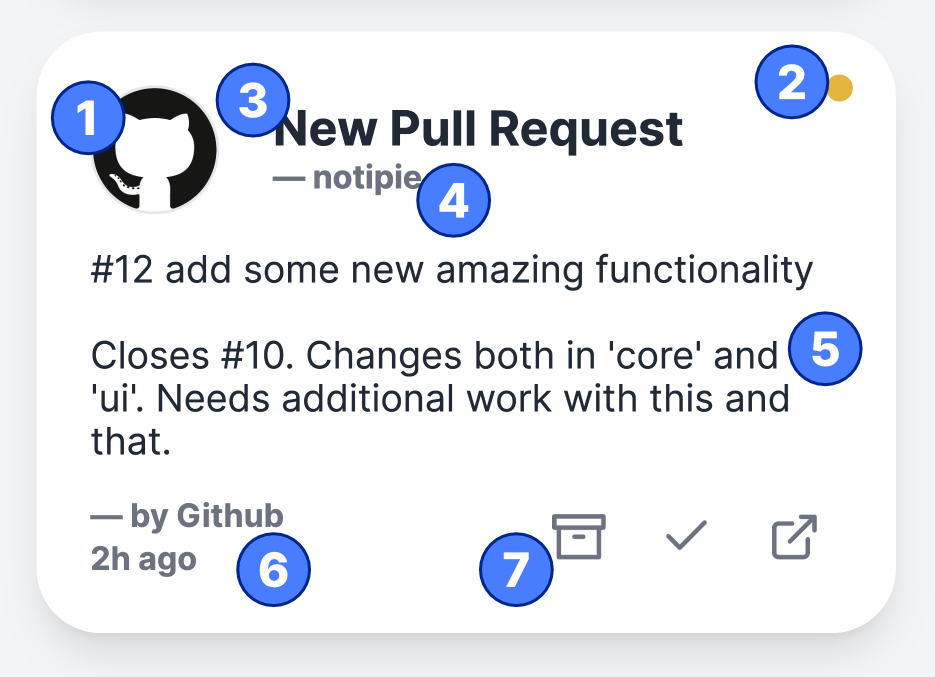
\includegraphics[width=10cm,keepaspectratio]{img/card_labeled.png}
      \caption{The card with labeled elements}
      \label{fig:card-with-labeled-elements}
\end{figure}

\begin{figure}[p]
      \centering
      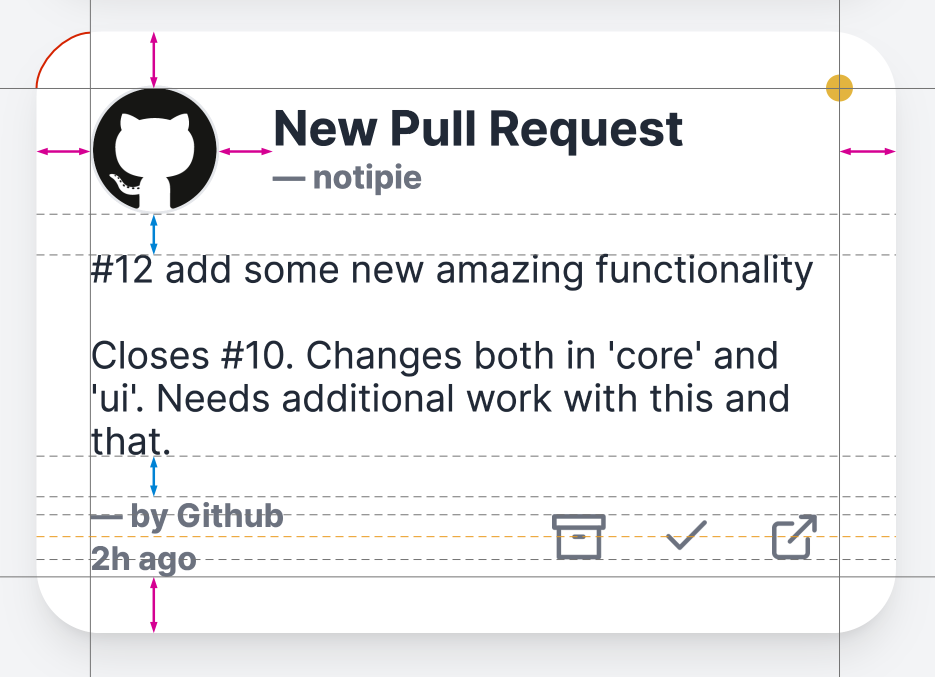
\includegraphics[width=10cm,keepaspectratio]{img/card_guides.png}
      \caption{The card with guides}
      \label{fig:card-with-guides}
\end{figure}

\subsection{UI component library}\label{ui-component-library}

When choosing the library for the UI components, I considered:

\begin{itemize}
  \item
    React\footnote{React, retrieved 2022-05-31. \url{https://reactjs.org/}},
  \item
    Vue.js\footnote{Vue.js, retrieved 2022-05-31. \url{https://vuejs.org/}},
    and
  \item
    Angular\footnote{Angular, retrieved 2022-05-31.
    \url{https://angular.io/}}.
\end{itemize}

All those libraries are very popular, so I chose React, because I had
the most experience with it in my professional work.

\subsection{UI networking}\label{ui-networking}

The nature of notifications required me to use
both REST data fetching and asynchronous data pushes from the backend.
For the latter, I decided to use WebSockets,
a standard defined in RFC6455~\cite{fette_rfc6455_2011}, and
RxJS~\cite{lesh_rxjs_2022}, an implementation of
ReactiveX library~\cite{gross_reactivex_2021}.

\subsubsection{REST data fetching}\label{rest-data-fetching}

I used simple REST~\cite{perrier_rest_2022} requests
for fetching the notifications
that are already on the backend server.
The standard Fetch browser API~\cite{perrier_fetch_2022}
was sufficient for the task.

\subsubsection{Reactive Raven}\label{reactive-raven}

This project~\cite{sewera_reactive_2022} was an experiment
on using RxJS for all real-time data fetching,
enabling the separation of concerns in the code,
and decoupling the state management implementation
from the networking implementation.

When searching for the optimal solution for pushing the data to the UI,
I came across two major solutions:

\begin{itemize}
  \item
        Redux Thunk~\cite{gaeraon_redux_2022-1} --
        enough for fetching data on user interaction,
        e.g., on a button click,
        but it provides virtually full implementation lock-in
        to the Redux store, and very little separation of concerns.
        Fetching data is an action dispatched on a store,
        so external communication and storing data are dependent on each other.
  \item
        Redux Saga~\cite{elouafi_redux_2022} --
        good for managing side effects with plain JavaScript,
        but it uses generator functions
        that yield a different type every time,
        so it is very problematic to use with strict TypeScript.
\end{itemize}

Both thunks and sagas did not provide the separation of concerns
I wanted to achieve.
Fetching or acting upon pushed data
is a different concern than storing it.

As a user,
I should not have to dispatch an action on a store
when I want to fetch data.
Of course, the data can be immediately stored after fetching,
but this behavior should be injected later,
so that there is no store implementation lock-in.

This separation of concerns enabled me to
migrate from Redux to Zustand as my \emph{store} implementation,
as described in the next section.

\subsection{State management in UI}\label{sec:state-management-in-ui}

To simplify the frontend code,
I needed to use a single source of truth for the data.
I used both Redux~\cite{gaeraon_redux_2022},
and Zustand~\cite{kato_zustand_2022} for this task
as \textit{store} implementations,
and Zustand came on top as a simpler solution for my application.

\subsubsection{Redux}\label{sec:redux}

Redux is great for big applications with lots of components.
Being one of the most popular state management libraries for React,
it was my first choice.
Unfortunately,
it required me to write a lot of boilerplate code,
and thus was not easily maintainable
for a smaller project like Notipie.

\subsubsection{Zustand}\label{sec:zustand}

Zustand is a lot simpler than Redux,
requires a lot less boilerplate code,
and was sufficient for my application.
I migrated to it in commit
\texttt{7677d13}\footfullcite{sewera_choreui_2022},
and it reduced the lines of code by over 200.
I did not, however, give up the connected components,
as they provide better testability and separation of concerns,
which is worth a bit extra code.

\addtocategory{commit}{sewera_choreui_2022}

\subsection{TypeScript in UI}\label{sec:typescript-in-ui}

I decided to use TypeScript in my project for the frontend part,
because of its type checking tools,
huge popularity,
and a growing demand for in on the job market.

\subsubsection{Choosing the language}\label{sec:choosing-the-language}

When choosing which language to use in the UI,
I considered a couple of options:

\begin{itemize}
      \item
            plain JavaScript,
      \item
            TypeScript,
      \item
            Elm, and
      \item
            CoffeeScript.
\end{itemize}

I immediately discarded the last two,
due to their smaller popularity,
compared to JavaScript or TypeScript.

The featureset of the language was also very important to me.
JavaScript is by far the most popular,
but it lacks type annotations or pre-runtime type checking.
TypeScript and Elm turned out to be winners in the type checking toolchain.

TypeScript also has a big advantage of being very similar to plain JavaScript,
so the transpiled code is very readable.

A big factor was general trend of language's popularity growth.
TypeScript was a clear winner in this scenario,
being third most loved language
and second most wanted language
in the Stack Overflow Developer Survey 2021~\cite{stack_overflow_2021_2021}.

It was only beaten by Rust and Clojure
in the \textit{Most Loved} section,
both of which are non-frontend languages,
and Python in the \textit{Most Wanted} section,
which is also not a frontend language.

Another report confirming the growing popularity of TypeScript
is Github Octoverse Report 2021~\cite{github_inc_2021_2021}.
Since 2017,
it beat
Ruby,
C,
C++,
C\#,
Shell, and
PHP
and is, as of 2021, the fourth top language on Github.

\subsubsection{Working with TypeScript}\label{sec:working-with-typescript}

Starting with TypeScript was fairly easy.
The toolchain was included in the project creation scripts.
Most dependencies had good TypeScript annotations,
or they were completely written in TypeScript,
which was very helpful for maintaining type safety.

Learning the language was also very easy.
I was already familiar with JavaScript,
so I only needed to learn the type annotations,
which were very intuitive to use.

\subsection{Build system}\label{build-system}

For the build and bundle software,
I wanted to use something modern,
with hot module reloading,
easy to use setup scripts,
customizable development server,
and short bundle times.

\subsubsection{Snowpack and Vite}\label{snowpack-and-vite}

I started with Snowpack~\cite{schott_snowpack_2021}
and used it until I decided to move to Vite~\cite{you_vite_2022}
in commit \texttt{c11bc35}\footnote{
  commit \texttt{c11bc35}, 2021.
    [Online]. (visited on 2022-05-31).
  \url{https://github.com/blazejsewera/notipie/commit/c11bc35370f512f35d522a55fcd216c1c80ea75a}
}.

Snowpack offered both hot module reloading and short bundle times,
however, there were some minor problems from time to time, the project
had a slow development, and the alternative, Vite did not seem to have
those problems.

I tried Vite in my other project, Reactive Raven\footnote{Reactive
  Raven, retrieved 2022-05-31.
  \url{https://github.com/blazejsewera/reactive-raven}}, and the
integration with React, TypeScript, Tailwind CSS, and other tools I used
was seamless, therefore I decided to migrate to it in Notipie as well.

On April 20th, 2022, Snowpack's maintainer stated in the project's
Readme document (commit \texttt{45456aa})\footnote{project's Readme
  document (commit \texttt{45456aa}), retrieved 2022-05-31.
  \url{https://github.com/FredKSchott/snowpack/blob/45456aa14978460afcb5ce20f7296556d22c7595/README.md}}
that they would no longer maintain the project and mentioned Vite as a
good alternative for it.



\clearpage % Always start a section from a new page
\section{Summary}
TODO: Summary

%---------------
% Bibliography
%---------------
\cleardoublepage
\printbibliography
\clearpage

% Acronym list
% TODO: Remember to sort acronyms alphabetically manually!
\acronymlist
\acronym{API}{Application Programming Interface}
\acronym{DI}{Dependency Injection}
\acronym{IDE}{Integrated Development Environment}
\acronym{REST}{Representational State Transfer}~\cite{perrier_rest_2022}
\acronym{TDD}{Test-Driven Development}

\vspace{0.8cm}

%------------------------------------------
% Lists of figures, tables, and appendices
%------------------------------------------
\pagestyle{plain}

\listoffigurestoc
\vspace{1cm}
\listoftablestoc
\vspace{1cm}
\listofappendicestoc

%-------------
% Appendices
%-------------

%% Figures and tables in appendices are not listed
% \captionsetup[figure]{list=no}
% \captionsetup[table]{list=no}

%% Example Appendix 1
% \clearpage
% \appendix{Appendix name 1}
% \begin{figure}[!h]
% 	\centering \includegraphics[width=0.5\linewidth]{logopw2.png}
% 	\caption{Obrazek w załączniku.}
% \end{figure}

%% Example Appendix 2
% \clearpage
% \appendix{Appendix name 2}
% \begin{table}[!h] \centering
%     \caption{Tabela w załączniku.}
%     \begin{tabular} {| c | c | r |} \hline
%         Kolumna 1       & Kolumna 2 & Liczba \\ \hline\hline
%         cell1           & cell2     & 60     \\ \hline
%         \multicolumn{2}{|r|}{Suma:} & 123,45 \\ \hline
%     \end{tabular}
% \end{table}

\end{document} % Goodnight
